% The equation of a plane $P$ passing through the intersection of two planes $P_{1}$ and $P_{2}$ is given by,
% \begin{align}
%    P : P_{1} + \lambda P_{2}\label{sep/2/27/eq1}
% \end{align}
\begin{lemma}
The equation of a plane passing through the intersection of two planes and given point will be\\
% \begin{align}
% P : P_{1} + \lambda P_{2}\label{sep/2/27/eq1}
% \end{align}
Let 
\begin{align}
P_1: \quad \vec{n_{1}}^T\vec{x}&=c_{1}\\ P_2: \quad  \vec{n_{2}}^T\vec{x}&=c_{2}
\end{align}
Then, 
\begin{align}
P: \quad \vec{n^T\vec{x}}&=c
\end{align}
%Point through which Plane $P$ is passing is $A$\\
where
\begin{align}
\label{sep/2/27/lemma}
\vec{n} &= \vec{n_{1}} + \brak{\frac{c_{1} - \vec{n_{1}}^T\vec{A}}{\vec{n_{2}}^T\vec{A}- c_{2}}}\vec{n_{2}}\\
c &= c_{1} + \brak{\frac{c_{1} - \vec{A}\vec{n_{1}}^T}{\vec{A}\vec{n_{2}}^T- c_{2}}}c_{2}
\end{align}
\end{lemma}
\begin{proof}
$P$ has the equation
\begin{align}
\vec{n_{1}}^T\vec{x} + \lambda\brak{\vec{n_{2}}^T\vec{x}} = c_{1} + \lambda\brak{c_{2}}\\
\implies \brak{\vec{n_{1}}+\lambda\vec{n_{2}}}^T\vec{x} = c_{1} + \lambda\brak{c_{2}}
\end{align}
Then
\begin{align}\label{sep/2/27/eq:12}
\vec{n} &= \vec{n_{1}} + \lambda\vec{n_{2}}\\
c &= c_{1} + \lambda c_{2}
\end{align}
Given that plane $P$ passes through point $\vec{A}$ then
\begin{align}
\brak{\vec{n_{1}}+\lambda\vec{n_{2}}}^T\vec{A} &= c_{1} + \lambda\brak{c_{2}}\\
\implies \lambda &= \frac{c_{1} - \vec{n_{1}}^T\vec{A}}{\vec{n_{2}}^T\vec{A}- c_{2}}
\end{align}
Substituting $\lambda$ in \eqref{sep/2/27/eq:12} yields \ref{sep/2/27/lemma}.
% \begin{align}
% \vec{n}^T &= \vec{n_{1}}^T + \brak{\frac{c_{1} - \vec{n_{1}}^T\vec{A}}{\vec{n_{2}}^T\vec{A}- c_{2}}}\vec{n_{2}}^T\\
% c &= c_{1} + \brak{\frac{c_{1} - \vec{n_{1}}^T\vec{A}}{\vec{n_{2}}^T\vec{A}- c_{2}}}c_{2}
% \end{align}
 \end{proof}
For the given problem 
\begin{align}
\vec{n_{1}}=\myvec{2\\2\\-3}\\
\vec{n_{2}} =\myvec{2\\5\\3}\\
c_{1} = 7\\
c_{2} = 9
\end{align}
By substituting the given values,
\begin{align}
\lambda &= \frac{10}{9}\\
\vec{n} &= \myvec{\frac{38}{9}\\\frac{68}{9}\\\frac{1}{3}}\\
c &= 17
\end{align}
So the equation of plane $P$ is given by
\begin{align}
\myvec{\frac{38}{9}&\frac{68}{9}&\frac{1}{3}}\vec{x} &= 17
\end{align}
See Fig. \ref{sep/2/27/fig:Line }.	
\begin{figure}[!ht]
\centering
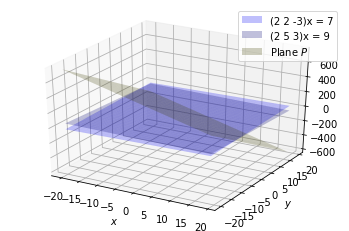
\includegraphics[ width=\columnwidth]{solutions/sep/2/27/Figure/EE3900_Assignment_4.png}
\caption{Plane $P$ passing through intersection of $P_{1}$ and $P_{2}$ and through a point $\vec{A}$}
\label{sep/2/27/fig:Line }	
\end{figure}


